%{{第七十七回}}{第七十七回}}

\chapter{俏丫鬟抱屈夭风流 美优伶斩情归水月}

{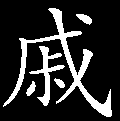
\includegraphics[width=3mm]{../Images/00005}\kaishu 司棋一事,前文着实写来,此却随笔收去;晴雯一事,前文不过带叙,此却竭力发挥。前文借晴雯一衬,文不寂寞;此文借司棋一引,文愈曲折。}

话说王夫人见中秋已过,凤姐病已比先减了,虽未大愈,可以出入行走得了,仍命大夫每日诊脉服药,又开了丸药方子来配调经养荣丸。因用上等人参二两,王夫人命人取时,翻寻了半日,只向小匣内寻了几枝簪挺粗细的。王夫人看了嫌不好,命再找去,又找了一大包须末出来。王夫人焦躁道:``用不着偏有,但用着了,再找不着。成日家我说叫你们查一查,都归拢在一处。你们白不听,就随手混撂。你们不知他的好处,用起来得多少换买来还不中使呢。''彩云道:``想是没了,就只有这个。上次那边的太太来寻了些去,太太都给过去了。''王夫人道:``没有的话,你再细找找。''彩云只得又去找,拿了几包药材来说:``我们不认得这个,请太太自看。除这个再没有了。''王夫人打开看时,也都忘了,不知都是什么药,并没有一枝人参。因一面遣人去问凤姐有无,凤姐来说:``也只有些参膏。芦须虽有几枝,也不是上好的,每日还要煎药里用呢。''王夫人听了,只得向邢夫人那里问去。
邢夫人说:``因上次没了,才往这里来寻,早已用完了。''王夫人没法,只得亲身过来请问贾母。贾母忙命鸳鸯取出当日所馀的来,竟还有一大包,皆有手指头粗细的,遂称二两与王夫人。王夫人出来交与周瑞家的拿去,令小厮送与医生家去,又命将那几包不能辨得的药也带了去,命医生认了,各包记号了来。{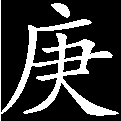
\includegraphics[width=3mm]{../Images/00004}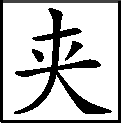
\includegraphics[width=3mm]{../Images/00012}\footnotesize \kaishu 此等皆家常细事,岂是揣摩得出者。}

一时,周瑞家的又拿了进来说:``这几包都各包好记上名字了。但这一包人参固然是上好的,\elegantpar{如今就连三十换也不能得这样的了}{积累},但年代太陈了。这东西比别的不同,凭是怎样好的,只过一百年后,便自己就成了灰了。如今这个虽未成灰,然已成了朽糟烂木,也无性力的了。请太太收了这个,倒不拘粗细,好歹再换些新的倒好。''王夫人听了,低头不语,半日才说:``这可没法了,只好去买二两来罢。''也无心看那些,只命:``都收了罢。''因向周瑞家的说:``你就去说给外头人们,拣好的换二两来。倘一时老太太问,你们只说用的是老太太的,不必多说。''周瑞家的方才要去时,宝钗因在坐,乃笑道:``姨娘且住。如今外头卖的人参都没好的。\elegantpar{虽有一枝全的,他们也必截做两三段,镶嵌上芦泡须枝,掺匀了好卖,看不得粗细。}{智商税,哎,奸猾商人}我们铺子里常和参行交易,如今我去和妈说了,叫哥哥去托个伙计过去和参行商议说明,叫他把未作的原枝好参兑二两来。不妨咱们多使几两银子,也得了好的。''王夫人笑道:``倒是你明白。就难为你亲自走一趟更好。''于是宝钗去了,半日回来说:``已遣人去,赶晚就有回信的。明日一早去配也不迟。''王夫人自是喜悦,因说道:```卖油的娘子水梳头',自来家里有好的,不知给了人多少。这会子轮到自己用,反倒各处求人去了。''说毕长叹。宝钗笑道:``这东西虽然值钱,究竟不过是药,原该济众散人才是。咱们比不得那没见世面的人家,得了这个,就珍藏密敛的。''{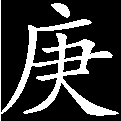
\includegraphics[width=3mm]{../Images/00004}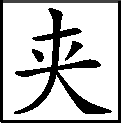
\includegraphics[width=3mm]{../Images/00012}\footnotesize \kaishu 调侃语。}王夫人点头道:``这话极是。''

一时宝钗去后,因见无别人在室,遂唤周瑞家的来,问前日园中搜检的事情可得个下落。周瑞家的是已和凤姐等人商议停妥,一字不隐,遂回明王夫人。王夫人听了,虽惊且怒,却又作难,因思司棋系迎春之人,皆系那边的人,只得令人去回邢夫人。周瑞家的回道:``前日那边太太嗔着王善保家的多事,打了几个嘴巴子,如今他也装病在家,不肯出头了。况且又是他外孙女儿,自己打了嘴,他只好装个忘了,日久平服了再说。如今我们过去回时,恐怕又多心,倒像似咱们多事似的。不如直把司棋带过去,一并连赃证与那边太太瞧了,不过打一顿配了人,再指个丫头来,岂不省事。如今白告诉去,那边太太再推三阻四的,又说`既这样你太太就该料理,又来说什么',岂不反耽搁了。倘那丫头瞅空寻了死,反不好了。如今看了两三天,人都有个偷懒的,倘一时不到,岂不倒弄出事来。''王夫人想了一想,说:``这也倒是。快办了这一件,再办咱们家的那些妖精。''

周瑞家的听说,会齐了那几个媳妇,先到迎春房里,回迎春道:``太太们说了,司棋大了,连日他娘求了太太,太太已赏了他娘配人,今日叫他出去,另挑好的与姑娘使。''说着,便命司棋打点走路。迎春听了,含泪似有不舍之意,因前夜已闻得别的丫鬟悄悄的说了原故,虽数年之情难舍,但事关风化,亦无可如何了。那司棋也曾求了迎春,实指望迎春能死保赦下的,只是迎春语言迟慢,耳软心活,是不能作主的。司棋见了这般,知不能免,因哭道:``姑娘好狠心!哄了我这两日,如今怎么连一句话也没有?''周瑞家的等说道:``你还要姑娘留你不成?便留下,你也难见园里的人了。依我们的好话,快快收了这样子,倒是人不知鬼不觉的去罢,大家体面些。''迎春含泪道:``我知道你干了什么大不是,我还十分说情留下,岂不连我也完了。你瞧入画也是几年的人,怎么说去就去了。自然不止你两个,想这园里凡大的都要去呢。依我说,将来终有一散,不如你各人去罢。''周瑞家的道:``所以到底是姑娘明白。明儿还有打发的人呢,你放心罢。''司棋无法,只得含泪与迎春磕头,和众姊妹告别,又向迎春耳根说:``好歹打听我要受罪,替我说个情儿,就是主仆一场!''迎春亦含泪答应:``放心。''

于是周瑞家的人等带了司棋出了院门,又命两个婆子将司棋所有的东西都与他拿着。走了没几步,后头只见绣橘赶来,一面也擦着泪,一面递与司棋一个绢包说:``这是姑娘给你的。主仆一场,如今一旦分离,这个与你作个想念罢。''司棋接了,不觉更哭起来了,又和绣橘哭了一回。周瑞家的不耐烦,只管催促,二人只得散了。司棋因又哭告道:``婶子大娘们,好歹略徇个情儿,如今且歇一歇,让我到相好的姊妹跟前辞一辞,也是我们这几年好了一场。''周瑞家的等皆各有事务,作这些事便是不得已了,况且又深恨他们素日大样,如今那里有工夫听他的话,因冷笑道:``我劝你走罢,别拉拉扯扯的了。我们还有正经事呢。谁是你一个衣包里爬出来的,辞他们作什么,他们看你的笑声还看不了呢。你不过是挨一会是一会罢了,难道就算了不成!依我快走罢。''一面说,一面总不住脚,直带着往后角门出去了。司棋无奈,又不敢再说,只得跟了出来。

可巧正值宝玉从外而入,一见带了司棋出去,又见后面抱着些东西,料着此去再不能来了。
因闻得上夜之事,又兼晴雯之病亦因那日加重,细问晴雯,又不说是为何。上日又见入画已去,今又见司棋亦走,不觉如丧魂魄一般,因忙拦住问道:``那里去?''周瑞家的等皆知宝玉素日行为,又恐唠叨误事,因笑道:``不干你事,快念书去罢。''宝玉笑道:``好姐姐们,且站一站,我有道理。''周瑞家的便道:``太太不许少捱一刻,又有什么道理。我们只知遵太太的话,管不得许多。''司棋见了宝玉,因拉住哭道:``他们做不得主,你好歹求求太太去。''宝玉不禁也伤心,含泪说道:``我不知你作了什么大事,晴雯也病了,如今你又去。都要去了,这却怎么的好。''{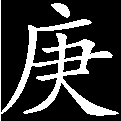
\includegraphics[width=3mm]{../Images/00004}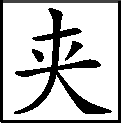
\includegraphics[width=3mm]{../Images/00012}\footnotesize \kaishu 宝玉之语全作囫囵意,最是极无味之语,偏是极浓极有情之语也。只合如此写方是宝玉,稍有真切则不是宝玉了。}周瑞家的发躁向司棋道:``你如今不是副小姐了,若不听话,我就打得你。别想着往日有姑娘护着,任你们作耗。越说着,还不好好走。如今和小爷们拉拉扯扯,成个什么体统!''那几个媳妇不由分说,拉着司棋便出去了。

宝玉又恐他们去告舌,恨的只瞪着他们,看已去远,方指着恨道:``奇怪,奇怪,怎么这些人只一嫁了汉子,染了男人的气味,就这样混帐起来,比男人更可杀了!''守园门的婆子听了,也不禁好笑起来,因问道:``这样说,\elegantpar{凡女儿个个是好的了,女人个个是坏的了}{宝玉眼里,也有,配穿红的,花的名字}?''宝玉点头道:``不错,不错!''婆子们笑道:``还有一句话我们糊涂不解,倒要请问请问。''方欲说时,只见几个老婆子走来,忙说道:``你们小心,传齐了伺候着。此刻太太亲自来园里,在那里查人呢。只怕还查到这里来呢。又吩咐快叫怡红院的晴雯姑娘的哥嫂来,在这里等着领出他妹妹去。''因笑道:``阿弥陀佛!今日天睁了眼,把这一个祸害妖精退送了,大家清净些。''宝玉一闻得王夫人进来清查,便料定晴雯也保不住了,早飞也似的赶了去,所以这后来趁愿之语竟未得听见。

宝玉及到了怡红院,只见一群人在那里,王夫人在屋里坐着,一脸怒色,见宝玉也不理。晴雯四五日水米不曾沾牙,恹恹弱息,如今现从炕上拉了下来,蓬头垢面,两个女人才架起来去了。王夫人吩咐,只许把他贴身衣服撂出去,馀者好衣服留下给好丫头们穿。又命把这里所有的丫头们都叫来一一过目。

原来王夫人自那日着恼之后,王善保家的就趁势告倒了晴雯。本处有人和园中不睦的,也就随机趁便下了些话。王夫人皆记在心中。因节间有事,故忍了两日,今日特来亲自阅人。一则为晴雯犹可,二则因竟有人指宝玉为由,说他大了,已解人事,都由屋里的丫头们不长进教习坏了。因这事更比晴雯一人较甚,{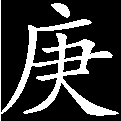
\includegraphics[width=3mm]{../Images/00004}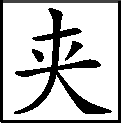
\includegraphics[width=3mm]{../Images/00012}\footnotesize \kaishu 暗伏一段。``更比'',觉烟迷雾罩之中更有无限溪山矣。}乃从袭人起以至于极小作粗活的小丫头们,个个亲自看了一遍。因问:``谁是和宝玉一日的生日?''本人不敢答应,老嬷嬷指道:``这一个蕙香,又叫作四儿的,是同宝玉一日生日的。''王夫人细看了一看,虽比不上晴雯一半,却有几分水秀。视其行止,聪明皆露在外面,且也打扮的不同。王夫人冷笑道:``这也是个不怕臊的。他背地里说的,同日生日就是夫妻。这可是你说的?打量我隔的远,都不知道呢。可知道我身子虽不大来,我的心耳神意时时都在这里。难道我通共一个宝玉,就白放心凭你们勾引坏了不成!''这个四儿见王夫人说着他素日和宝玉的私语,不禁红了脸,低头垂泪。王夫人即命也快把他家的人叫来,领出去配人。又问:``谁是耶律雄奴?''老嬷嬷们便将芳官指出。王夫人道:``唱戏的女孩子,自然是狐狸精了!上次放你们,你们又懒待出去,可就该安分守己才是。你就成精鼓捣起来,调唆着宝玉无所不为。''芳官哭辩道:``并不敢调唆什么。''王夫人笑道:``你还强嘴。我且问你,前年我们往皇陵上去,是谁调唆宝玉要柳家的丫头五儿了?幸而那丫头短命死了,不然进来了,你们又连伙聚党遭害这园子呢。你连你干娘都欺倒了,岂止别人!''因喝命:``唤他干娘来领去,就赏他外头自寻个女婿去吧。把他的东西一概给他。''又吩咐上年凡有姑娘们分的唱戏的女孩子们,一概不许留在园里,都令其各人干娘带出,自行聘嫁。一语传出,这些干娘皆感恩趁愿不尽,都约齐与王夫人磕头领去。

王夫人又满屋里搜检宝玉之物。凡略有眼生之物,一并命收的收,卷的卷,着人拿到自己房内去了。因说:``这才干净,省得旁人口舌。''因又吩咐袭人麝月等人:``你们小心!往后再有一点分外之事,我一概不饶。因叫人查看了,今年不宜迁挪,暂且挨过今年,明年一并给我仍旧搬出去心净。''{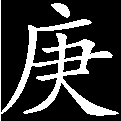
\includegraphics[width=3mm]{../Images/00004}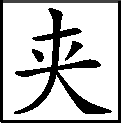
\includegraphics[width=3mm]{../Images/00012}\footnotesize \kaishu 一段神奇鬼讶之文不知从何想来,王夫人从来未理家务,岂不一木偶哉?且前文隐隐约约已有无限口舌,浸润之谮原非一日矣。若无此一番更变,不独终无散场之局,且亦大不近乎情理。况此亦皆余旧日目睹亲闻,作者身历之现成文字,非捏造而成者,故迥不与小说之离合悲欢窠臼相对。想遭零落之大族儿子见此,虽事各有殊,然其情理似亦有默契于心者焉。此一段不独批此,直从抄检大观园及贾母对月兴尽生悲皆可附者也。}说毕,茶也不吃,遂带领众人又往别处去阅人。暂且说不到后文。

如今且说宝玉只当王夫人不过来搜检搜检,无甚大事,谁知竟这样雷嗔电怒的来了。所责之事皆系平日之语,一字不爽,料必不能挽回的。虽心下恨不能一死,但王夫人盛怒之际,自不敢多言一句,多动一步,一直跟送王夫人到沁芳亭。王夫人命:``回去好生念念那书,仔细明儿问你。才已发下恨了。''宝玉听如此说,方回来,一路打算:``谁这样犯舌?况这里事也无人知道,如何就都说着了。''一面想,一面进来,只见袭人在那里垂泪。且去了第一等的人,岂不伤心,便倒在床上也哭起来。袭人知他心内别的还犹可,独有晴雯是第一件大事,乃推他劝道:``哭也不中用了。你起来我告诉你,晴雯已经好了,他这一家去,倒心净养几天。你果然舍不得他,等太太气消了,你再求老太太,慢慢的叫进来也不难。不过太太偶然信了人的诽言,一时气头上如此罢了。''宝玉哭道:``我究竟不知晴雯犯了何等滔天大罪!''{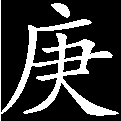
\includegraphics[width=3mm]{../Images/00004}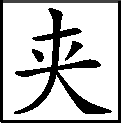
\includegraphics[width=3mm]{../Images/00012}\footnotesize \kaishu 余亦不知。盖此等冤实非晴雯一人也。}袭人道:``太太只嫌他生的太好了,未免轻佻些。在太太是深知这样美人似的人必不安静,所以恨嫌他,像我们这粗粗笨笨的倒好。''宝玉道:``这也罢了。咱们私自顽话怎么也知道了?又没外人走风的,这可奇怪。''袭人道:``你有甚忌讳的,一时高兴了,你就不管有人无人了。我也曾使过眼色,也曾递过暗号,倒被那别人已知道了,你反不觉。''宝玉道:``怎么人人的不是太太都知道,单不挑出你和麝月秋纹来?''袭人听了这话,心内一动,低头半日,无可回答,因便笑道:``正是呢。若论我们也有顽笑不留心的孟浪去处,怎么太太竟忘了?想是还有别的事,等完了再发放我们,也未可知。''宝玉笑道:``你是头一个出了名的至善至贤之人,他两个又是你陶冶教育的,焉得还有孟浪该罚之处!只是芳官尚小,过于伶俐些,未免倚强压倒了人,惹人厌。四儿是我误了他,还是那年我和你拌嘴的那日起,叫上来作些细活,未免夺占了地位,故有今日。只是晴雯也是和你一样,从小儿在老太太屋里过来的,虽然他生得比人强,也没甚妨碍去处。就是他的性情爽利,口角锋芒些,究竟也不曾得罪你们。想是他过于生得好了,反被这好所误。''说毕,复又哭起来。

袭人细揣此话,好似宝玉有疑他之意,竟不好再劝,因叹道:``天知道罢了。此时也查不出人来了,白哭一会子也无益。倒是养着精神,等老太太喜欢时,回明白了再要来是正理。''宝玉冷笑道:``你不必虚宽我的心。等到太太平服了再瞧势头去要时,知他的病等得等不得。他自幼上来娇生惯养,何尝受过一日委屈。连我知道他的性格,还时常冲撞了他。他这一下去,就如同一盆才抽出嫩箭来的兰花送到猪窝里去一般。况又是一身重病,里头一肚子的闷气。他又没有亲爷热娘,只有一个醉泥鳅姑舅哥哥。他这一去,一时也不惯的,那里还等得几日。知道还能见他一面两面不能了!''说着又越发伤心起来。袭人笑道:``可是你`只许州官放火,不许百姓点灯'。我们偶然说一句略妨碍些的话,就说是不利之谈,你如今好好的咒他,是该的了!他便比别人娇些,也不至这样起来。''宝玉道:``不是我妄口咒他,今年春天已有兆头的。''袭人忙问何兆。宝玉道:``这阶下好好的一株海棠花,竟无故死了半边,我就知有异事,果然应在他身上。''袭人听了,又笑起来,因说道:``我待不说,又撑不住,你太也婆婆妈妈的了。这样的话,岂是你读书的男人说的。草木怎又关系起人来?{若不婆婆妈妈的,真也成了个呆子了。}\href{../Text/part0081_split_000.html\#lnkback_1_a}{\textsuperscript{①}}''

宝玉叹道:``你们那里知道,不但草木,凡天下之物,皆是有情有理的,也和人一样,得了知己,便极有灵验的。若用大题目比,就有孔子庙前之桧,坟前之蓍,诸葛祠前之柏,岳武穆坟前之松。这都是堂堂正大随人之正气,千古不磨之物。世乱则萎,世治则荣,几千百年了,枯而复生者几次。这岂不是兆应?小题目比,就有杨太真沉香亭之木芍药,端正楼之相思树,王昭君冢上之草,岂不也有灵验。所以这海棠亦应其人欲亡,故先就死了半边。''袭人听了这篇痴话,又可笑,又可叹,因笑道:``真真的这话越发说上我的气来了。那晴雯是个什么东西,就费这样心思,比出这些正经人来!还有一说,他纵好,也灭不过我的次序去。便是这海棠,也该先来比我,也还轮不到他。想是我要死了。''宝玉听说,忙握他的嘴,劝道:``这是何苦!一个未清,你又这样起来。罢了,再别提这事,别弄的去了三个,又饶上一个。''袭人听说,心下暗喜道:``若不如此,你也不能了局。''宝玉乃道:``从此休提起,全当他们三个死了,不过如此。况且死了的也曾有过,也没见我怎么样,此一理也。{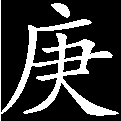
\includegraphics[width=3mm]{../Images/00004}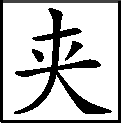
\includegraphics[width=3mm]{../Images/00012}\footnotesize \kaishu 宝玉至终一着全作如是想,所以始于情终于悟者。既能终于悟而止,则情不得滥漫而涉于淫佚之事矣。一人前事,一人了法,皆非``弃竹而复悯笋''之意。}如今且说现在的,倒是把他的东西,作瞒上不瞒下,悄悄的打发人送出去与了他。再或有咱们常时积攒下的钱,拿几吊出去给他养病,也是你姊妹好了一场。''袭人听了,笑道:``你太把我们看的又小器又没人心了。这话还等你说,我才已将他素日所有的衣裳以至各什各物总打点下了,都放在那里。如今白日里人多眼杂,又恐生事,且等到晚上,悄悄的叫宋妈给他拿出去。我还有攒下的几吊钱也给他罢。''宝玉听了,感谢不尽。袭人笑道:``我原是久已出了名的贤人,连这一点子好名儿还不会买来不成!''宝玉听他方才的话,忙陪笑抚慰一时。晚间果密遣宋妈送去。

宝玉将一切人稳住,便独自得便出了后角门,央一个老婆子带他到晴雯家去瞧瞧。先是这婆子百般不肯,只说怕人知道,``回了太太,我还吃饭不吃饭!''无奈宝玉死活央告,又许他些钱,那婆子方带了他来。这晴雯当日系赖大家用银子买的,那时晴雯才得十岁,尚未留头。因常跟赖嬷嬷进来,贾母见他生得伶俐标致,十分喜爱。故此赖嬷嬷就孝敬了贾母使唤,后来所以到了宝玉房里。这晴雯进来时,也不记得家乡父母。只知有个姑舅哥哥,专能庖宰,也沦落在外,故又求了赖家的收买进来吃工食。赖家的见晴雯虽到贾母跟前,千伶百俐,嘴尖性大,却倒还不忘旧,{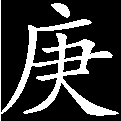
\includegraphics[width=3mm]{../Images/00004}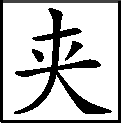
\includegraphics[width=3mm]{../Images/00012}\footnotesize \kaishu 只此一句便是晴雯正传。可知晴雯为聪明风流所害也。一篇为晴雯写传,是哭晴雯也。非哭晴雯,乃哭风流也。}故又将他姑舅哥哥收买进来,把家里一个女孩子配了他。成了房后,谁知他姑舅哥哥一朝身安泰,就忘却当年流落时,任意吃死酒,家小也不顾。偏又娶了个多情美色之妻,见他不顾身命,不知风月,一味死吃酒,便不免有蒹葭倚玉之叹,红颜寂寞之悲。又见他\elegantpar{器量宽宏}{鲍二一般的气量},{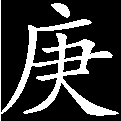
\includegraphics[width=3mm]{../Images/00004}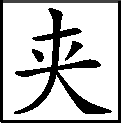
\includegraphics[width=3mm]{../Images/00012}\footnotesize \kaishu 趣极!``器量宽宏''如此用,真扫地矣。}并无嫉衾妒枕之意,这媳妇遂恣情纵欲,满宅内便延揽英雄,收纳材俊,上上下下竟有一半是他\elegantpar{考试}{考试如此用,啊}过的。若问他夫妻姓甚名谁,便是上回贾琏所接见的多浑虫灯姑娘儿的便是了。{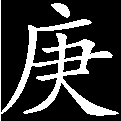
\includegraphics[width=3mm]{../Images/00004}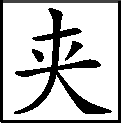
\includegraphics[width=3mm]{../Images/00012}\footnotesize \kaishu 奇奇怪怪,左盘右旋,千丝万线,皆自一体也。}目今晴雯只有这一门亲戚,所以出来就在他家。

此时多浑虫外头去了,那灯姑娘吃了饭去串门子,只剩下晴雯一人,在外间房内\elegantpar{爬}{一字写尽}着。{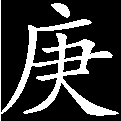
\includegraphics[width=3mm]{../Images/00004}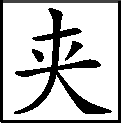
\includegraphics[width=3mm]{../Images/00012}\footnotesize \kaishu 总哭晴雯。}宝玉命那婆子在院门了哨,他独自掀起草帘{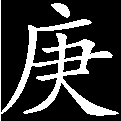
\includegraphics[width=3mm]{../Images/00004}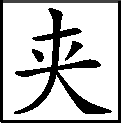
\includegraphics[width=3mm]{../Images/00012}\footnotesize \kaishu ``草帘''。}进来,一眼就看见晴雯睡在芦席土炕上,{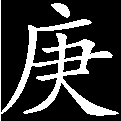
\includegraphics[width=3mm]{../Images/00004}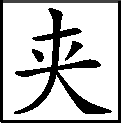
\includegraphics[width=3mm]{../Images/00012}\footnotesize \kaishu ``芦席土炕''。}幸而衾褥还是旧日铺的。心内不知自己怎么才好,因上来含泪伸手轻轻拉他,悄唤两声。当下晴雯又因着了风,又受了他哥嫂的歹话,病上加病,嗽了一日,才朦胧睡了。忽闻有人唤他,强展星眸,一见是宝玉,又惊又喜,又悲又痛,忙一把死攥住他的手。哽咽了半日,方说出半句话来:``我只当不得见你了。''接着便嗽个不住。宝玉也只有哽咽之分。

晴雯道:``阿弥陀佛,你来的好,且把那茶倒半碗我喝。渴了这半日,叫半个人也叫不着。''宝玉听说,忙拭泪问:``茶在那里?''晴雯道:``那炉台上就是。''宝玉看时,虽有个黑沙吊子,却不像个茶壶。只得桌上去拿了一个碗,也甚大甚粗,不像个茶碗,未到手内,先就闻得油膻之气。{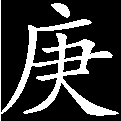
\includegraphics[width=3mm]{../Images/00004}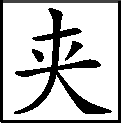
\includegraphics[width=3mm]{../Images/00012}\footnotesize \kaishu 不独为晴雯一哭,且为宝玉一哭亦可。}宝玉只得拿了来,先拿些水洗了两次,复又用水汕过,方提起沙壶斟了半碗。看时,绛红的,也太不成茶。晴雯扶枕道:``快给我喝一口罢!这就是茶了。那里比得咱们的茶!''宝玉听说,先自己尝了一尝,并无清香,且无茶味,只一味苦涩,略有茶意而已。尝毕,方递与晴雯。只见晴雯如得了甘露一般,一气都灌下去了。宝玉心下暗道:``往常那样好茶,他尚有不如意之处;今日这样。看来,可知古人说的`饱饫烹宰,饥餍糟糠',又道是`饭饱弄粥',可见都不错了。''{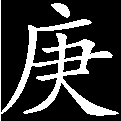
\includegraphics[width=3mm]{../Images/00004}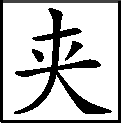
\includegraphics[width=3mm]{../Images/00012}\footnotesize \kaishu 妙!通篇宝玉最恶书者,每因女子之所历始信其可,此谓触类旁通之妙诀矣。}一面想,一面流泪问道:``你有什么说的,趁着没人告诉我。''晴雯呜咽道:``有什么可说的!不过挨一刻是一刻,挨一日是一日。我已知横竖不过三五日的光景,就好回去了。只是一件,我死也不甘心的:我虽生的比别人略好些,并没有私情密意勾引你怎样,如何一口死咬定了我是个狐狸精!我太不服。今日既已担了虚名,而且临死,不是我说一句后悔的话,早知如此,我当日也另有个道理。不料痴心傻意,只说大家横竖是在一处。不想平空里生出这一节话来,有冤无处诉。''说毕又哭。

宝玉拉着他的手,只觉瘦如枯柴,腕上犹戴着四个银镯,因泣道:``且卸下这个来,等好了再戴上罢。''因与他卸下来,塞在枕下。又说:``可惜这两个指甲,好容易长了二寸长,这一病好了,又损好些。''晴雯拭泪,就伸手取了剪刀,将左手上两根葱管一般的指甲齐根铰下;又伸手向被内将贴身穿着的一件旧红绫袄脱下,并指甲都与宝玉道:``这个你收了,以后就如见我一般。快把你的袄儿脱下来我穿。我将来在棺材内独自躺着,也就像还在怡红院的一样了。论理不该如此,只是担了虚名,我可也是无可如何了。''宝玉听说,忙宽衣换上,藏了指甲。晴雯又哭道:``回去他们看见了要问,不必撒谎,就说是我的。既担了虚名,越性如此,也不过这样了。''{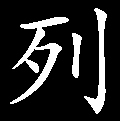
\includegraphics[width=3mm]{../Images/00007}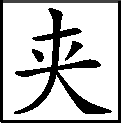
\includegraphics[width=3mm]{../Images/00012}\footnotesize \kaishu 晴雯此举胜袭人多矣,真一字一哭也,又何必鱼水相得而后为情哉?}

一语未了,只见他嫂子笑嘻嘻掀帘进来,道:``好呀,你两个的话,我已都听见了。''又向宝玉道:``你一个作主子的,跑到下人房里作什么?看我年轻又俊,敢是来调戏我么?''宝玉听说,吓的忙陪笑央道:``好姐姐,快别大声。他伏侍我一场,我私自来瞧瞧他。''灯姑娘便一手拉了宝玉进里间来,笑道:``你不叫嚷也容易,只是依我一件事。''说着,便坐在炕沿上,却紧紧的将宝玉搂入怀中。宝玉如何见过这个,心内早突突的跳起来了,急的满面红涨,又羞又怕,只说:``好姐姐,别闹。''{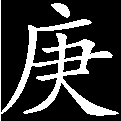
\includegraphics[width=3mm]{../Images/00004}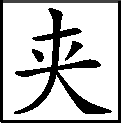
\includegraphics[width=3mm]{../Images/00012}\footnotesize \kaishu 如闻如见,``别闹''二字活跳。}灯姑娘乜斜醉眼,笑道:``呸!成日家听见你风月场中惯作工夫的,怎么今日就反讪起来。''宝玉红了脸,笑道:``\elegantpar{姐姐放手,有话咱们好说。}{海棠花,指晴雯,桃花指袭人}外头有老妈妈,听见什么意思。''灯姑娘笑道:``我早进来了,却叫婆子去园门等着呢。我等什么似的,今儿等着了你。虽然闻名,不如见面,空长了一个好模样儿,竟是没药信的炮仗,只好装幌子罢了,倒比我还发讪怕羞。可知人的嘴一概听不得的。就比如方才我们姑娘下来,我也料定你们素日偷鸡盗狗的。我进来一会在窗下细听,屋内只你二人,若有偷鸡盗狗的事,岂有不谈及于此,谁知你两个竟还是各不相扰。可知天下委屈事也不少。如今我反后悔错怪了你们。既然如此,你但放心。以后你只管来,我也不罗唣你。''

宝玉听说,才放下心来,方起身整衣央道:``好姐姐,你千万照看他两天。我如今去了。''说毕出来,又告诉晴雯。二人自是依依不舍,也少不得一别。晴雯知宝玉难行,遂用被蒙头,总不理他,宝玉方出来。意欲到芳官、四儿处去,无奈天黑,出来了半日,恐里面人找他不见,又恐生事,遂且进园来了,明日再作计较。因乃至后角门,小厮正抱铺盖,里边嬷嬷们正查人,若再迟一步也就关了。

宝玉进入园中,且喜无人知道。到了自己房内,告诉袭人只说在薛姨妈家去的,也就罢了。一时铺床,袭人不得不问今日怎么睡。宝玉道:``不管怎么睡罢了。''原来这一二年间袭人因王夫人看重了他了,越发自要尊重。凡背人之处,或夜晚之间,总不与宝玉狎昵,较先幼时反倒疏远了。况虽无大事办理,然一应针线并宝玉及诸小丫头们凡出入银钱衣履什物等事,也甚烦琐;且有吐血旧症虽愈,然每因劳碌风寒所感,即嗽中带血,故迩来夜间总不与宝玉同房。宝玉夜间常醒,又极胆小,每醒必唤人。因晴雯睡卧警醒,且举动轻便,故夜晚一应茶水起坐呼唤之任皆悉委他一人,所以宝玉外床只是他睡。今他去了,袭人只得要问,因思此任比日间紧要之意。宝玉既答不管怎样,袭人只得还依旧年之例,遂仍将自己铺盖搬来设于床外。

宝玉发了一晚上呆。{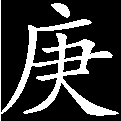
\includegraphics[width=3mm]{../Images/00004}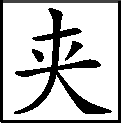
\includegraphics[width=3mm]{../Images/00012}\footnotesize \kaishu 一句足矣。}及催他睡下,袭人等也都睡后,听着宝玉在枕上长吁短叹,复去翻来,直至三更以后。方渐渐的安顿了,略有齁声。袭人方放心,也就朦胧睡着。没半盏茶时,只听宝玉叫``晴雯''。袭人忙睁开眼连声答应,问作什么。宝玉因要吃茶。袭人忙下去向盆内蘸过手,从暖壶内倒了半盏茶来吃过。宝玉乃笑道:{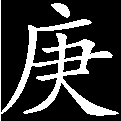
\includegraphics[width=3mm]{../Images/00004}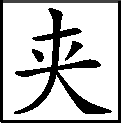
\includegraphics[width=3mm]{../Images/00012}\footnotesize \kaishu ``笑''字好极,有文章,盖恐冷落袭人也。}``我近来叫惯了他,却忘了是你。''袭人笑道:``他一乍来时你也曾睡梦中直叫我,半年后才改了。我知道这晴雯人虽去了,这两个字只怕是不能去的。''说着,大家又卧下。宝玉又翻转了一个更次,至五更方睡去时,只见晴雯从外头走来,仍是往日形景,进来笑向宝玉道:``你们好生过罢,我从此就别过了。''说毕,翻身便走。宝玉忙叫时,又将袭人叫醒。袭人还只当他惯了口乱叫,却见宝玉哭了,说道:``晴雯死了。''袭人笑道:``这是那里的话!你就知道胡闹,被人听着什么意思。''宝玉那里肯听,恨不得一时亮了就遣人去问信。

及至天亮时,就有王夫人房里小丫头立等叫开前角门传王夫人的话:``即时叫起宝玉,快洗脸,换了衣裳快来,因今儿有人请老爷寻秋赏桂花,老爷因喜欢他前儿作得诗好,故此要带他们去。这都是太太的话,一句别错了。你们快飞跑告诉他去,立逼他快来,老爷在上屋里还等他吃面茶呢。环哥儿已来了。快跑,快跑。再着一个人去叫兰哥儿,也要这等说。''里面的婆子听一句,应一句,一面扣扭子,一面开门。一面早有两三个人一行扣衣,一行分头去了。

袭人听得叩院门,便知有事,忙一面命人问时,自己已起来了。听得这话,促人来舀了面汤,催宝玉起来盥漱。他自去取衣。因思跟贾政出门,便不肯拿出十分出色的新鲜衣履来,只拿那二等成色的来。宝玉此时亦无法,只得忙忙的前来。果然贾政在那里吃茶,十分喜悦。宝玉忙行了省晨之礼。贾环贾兰二人也都见过宝玉。贾政命坐吃茶,向环兰二人道:``宝玉读书不如你两个,论题联和诗这种聪明,你们皆不及他。今日此去,未免强你们做诗,宝玉须听便助他们两个。''王夫人等自来不曾听见这等考语,真是意外之喜。

一时候他父子二人等去了,方欲过贾母这边来时,就有芳官等三个的干娘走来,回说:``芳官自前日蒙太太的恩典赏了出去,他就疯了似的,茶也不吃,饭也不用,勾引上藕官、蕊官,三个人寻死觅活,只要剪了头发做尼姑去。我只当是小孩子家一时出去不惯也是有的,不过隔两日就好了。谁知越闹越凶,打骂着也不怕。实在没法,所以来求太太,或是就依他们做尼姑去,或教导他们一顿,赏给别人作女儿去罢,我们也没这福。''王夫人听了道:``胡说!那里由得他们起来,佛门也是轻易人进去的!每人打一顿给他们,看还闹不闹了!''

当下因八月十五日各庙内上供去,皆有各庙内的尼姑来送供尖之例,王夫人曾于十五日就留下水月庵的智通与地藏庵的圆信住两日,至今日未回,听得此信,巴不得又拐两个女孩子去作活使唤,因都向王夫人道:``咱们府上到底是善人家。因太太好善,所以感应得这些小姑娘们皆如此。虽说佛门轻易难入,也要知道佛法平等。我佛立愿,原是一切众生无论鸡犬皆要度他,无奈迷人不醒。若果有善根能醒悟,即可以超脱轮回。所以经上现有虎狼蛇虫得道者就不少。如今这两三个姑娘既然无父无母,家乡又远,他们既经了这富贵,又想从小儿命苦入了这风流行次,将来知道终身怎么样,所以苦海回头,出家修修来世,也是他们的高意。太太倒不要限了善念。''

王夫人\elegantpar{原是个好善的}{虚伪仁义,常假佛道。},先听彼等之语不肯听其自由者,因思芳官等不过皆系小儿女一时不遂之谈,\href{../Text/part0081_split_000.html\#lnkback_2_a}{\textsuperscript{②}}恐将来熬不得清净,反致获罪。今听这两个拐子的话大近情理;且近日家中多故,又有邢夫人遣人来知会,明日接迎春家去住两日,以备人家相看;且又有官媒婆来求说探春等事,心绪正烦,那里着意在这些小事上。既听此言,便笑答道:``你两个既这等说,你们就带了作徒弟去如何?''两个姑子听了,念一声佛道:``善哉!善哉!若如此,可是你老人家阴德不小。''说毕,便稽首拜谢。王夫人道:``既这样,你们问他们去。若果真心,即上来当着我拜了师父去罢。''

这三个女人听了出去,果然将他三人带来。王夫人问之再三,他三人已是立定主意,遂与两个姑子叩了头,又拜辞了王夫人。王夫人见他们意皆决断,知不可强了,反倒伤心可怜,忙命人取了些东西来赍赏了他们,又送了两个姑子些礼物。从此芳官跟了水月庵的智通,蕊官、藕官二人跟了地藏庵的圆信,各自出家去了。再听下回分解。

{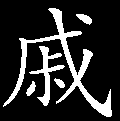
\includegraphics[width=3mm]{../Images/00005}\kaishu 总评:看晴雯与宝玉永绝一段,的是消魂文字;看宝玉几番呆论,真是至诚种子;看宝玉给晴雯斟茶,又真是呆公子。前文叙袭人奔丧时,宝玉夜来吃茶,先呼袭人,此又夜来吃茶,先呼晴雯。字字龙跳天门,虎卧凤阙;语语婴儿恋母,稚鸟寻巢。}

% {\href{../Text/part0081_split_000.html\#navto_1_a}{①}按:此句各本均为正文,网友娄员外提出疑是批语混入,近是。}

% {\href{../Text/part0081_split_000.html\#navto_2_a}{②}原作``一时不遂之但'',另笔点去``之''字,旁添``心故有此意''。诸本均作``不遂之谈'',``但''或系``谈''的音讹。唯``不遂之谈''略显生硬,是否的当,有待推敲。而底本旁改文字显非原文,暂从诸本改。}
